\section{Multi-band Adaptation Model}
\label{sec:model}
In this section, we introduce the pathloss and explain the potential gain of multiband adaptation in theory. The path loss shows a generally increasing trend with distance from the base,and related to the wavelength the decibel path loss can be presented as:\cite{erceg1999empirically}

\begin{equation}
PL=20log_{10}(4\pi d_0/\lambda)+10\gamma log_{10}(d/d_0)+s
\end{equation}

In an ideal channel, if the received signal is the same among all the bands, the performance should be the same. It is a reasonable assumption verified by experiments on the emulator. The performance across different bands in different received signal shows as: {fixme insert throughput vs rssi in bypass}

And also due to the limitation of FCC, the transmitting power of an Access Point is restricted. In the limited Acess range, the path loss of different bands are varying according to their wavelength. Without considering other factors, the difference of received signal makes the performance vary in different bands. Then, for a location, there is room to improve the performance in switching band.

Another problem for wireless communication is the utility level of a channel. Most of the wifi devices are working in 2.4GHz and 5GHz as 802.11 standard. 
Our method is to employ accumulate information in a time slot to quantify the channel state. The difference in crowd level of wireless channel also provide room for performance improvement in switching band.  
%In this section, we exploit channel dynamic and accumulate information in contextual data and develop band adaptation frame for dynamic environments.Through the proposed framework, we improve the throughput of a pair of multi-radio nodes according the given context. While in this paper we focus on the application to band adaptation to show gains, the framwork has other possible applications to transmission parameter adaptation based on context information. 


\subsection{Problem Formulation}
\label{subsec:problem}
The objective of this work is to introduce a way to predict the performance of multi-bands based on limited information of a single band. 
One step is to demonstrate the improvements in performance by leveraging information of ideal channels to make band adapatation decisions. 
As noted before, the context information we consider is the channel type, measured received signal strength, received bytes, background noise and channel interference. 
The channel type indicates the propagation and fading characteristics between the transmitter and receiver. Many factors(e.g., multi-path, path loss, and shadowing) have a substantial influence on the characteristics of the channel type.FIXME{citation of Hui paper} However, in this paper, we assume the channel type to be a static channel type across all the wireless bands. We use the defination of ITU channels, which are widely accepted as representative channel types for urban dan suburban settings \cite{recommendation19971225}. Moreover, noise and interference gradually changes in the field. The gradually changing process makes it possible to seperate the noise, and even the interference from time varying experiments. 
%The objective of this work is to demonstrate the improvements in performance by leveraging information of ideal channels to make band adapatation decisions. As noted before, the context information we consider is the channel type, measured received signal strength, received bytes, background noise and channel interference. The channel type indicates the propagation and fading characteristics between the transmitter and receiver. Many factors(e.g., multi-path, path loss, and shadowing) have a substantial influence on the characteristics of the channel type.FIXME{citation of Hui paper} However, in this paper, we assume the channel type to be a static channel type across all the wireless bands. We use the defination of ITU channels, which are widely accepted as representative channel types for urban dan suburban settings \cite{recommendation19971225}. Moreover, noise and interference gradually changes in the field. The gradually changing process makes it possible to seperate the noise, and even the interference from time varying experiments. 

So far, there is no work has done for such multi-band adaptation. 
Some multi-channel adaptation and rate adaptation scenarios are focus on \emph{Dynamic Channel State} as represented by \cite{cordeiro2007c,MOAR}:. 

\begin{equation}
f(SNR,Context-Aware\, Info) \rightarrow Channel
\end{equation}

which assumes that the performance is only related to the channel dynamic information. However, in our approach, we consider the intereference of channel state as a factor of statistics of time. The intereference factor gradually changing process makes the statistics have an embedded temporal correlation. We adapt the transmission band for each scenario based on the contextual information and the temporal correlation. 


In this paper, we involve a factor \emph{Activity Level} to the framework. For our case, the multi-band adaptation can be simply represented as:

\begin{equation}
f(SNR,Activity\, Level,Context-Aware\, Info) \rightarrow Band
\end{equation}

The new factor \emph{Activity \, Level} is defined as a statistics of band occupacied time ratio. Through the temporal correlation parameter, the prediction of the performance could match in-field system better than only consider the dynamic channel state.

\begin{figure}
\centering
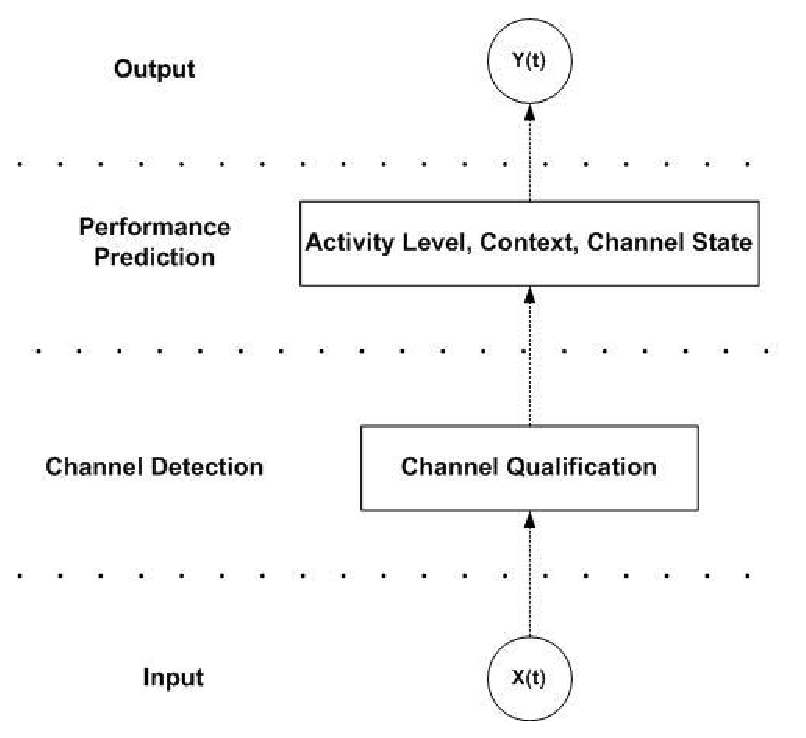
\includegraphics[width=85mm]{figure/multiband_framework}
\caption{Multiband framework.}
\label{fig:multiframe}
\end{figure}





\subsection{Context-Aware Information}

%1,what is context info


Contexts, which defines various operating situations. Depending on a context, the wireless device changes its operational 
behavior in accordance with a defined profile, when a context parameter changes \cite{phillips2004wireless}. Context is a database include the knowledge the system stored or learned from the experiments or activities. Based on tons of measurement under different parameters, a relationship between performance and system parameters can be created. In our band adaptation framework, the collected contextual information is the input to the multi-band adaptaion model. In the ideal channel context information, for each given set of bands, SNR, the context table can represent ideal throughput for each bands. 

%2,how others use the info Fixme
Context-aware information is the experience of a transmitor receiver pair. The performance of a system in the past can help transmiter to find the optimal rate/band based on the parameter collected by the receiver. Such as in FARA algroithm, the receiver uses an SNR characterization table that lists the minimum SNR required for a particular combination of modulation and coding rate\cite{rahul2009frequency}. 
Context-Aware information show a way to map the channel states to the performance.
%3,how we use the info

In our band adaptation framework, the collected contextual information is the input to the multi-band adaptaion model. In the ideal channel context information, for each given set of bands, SNR, the context table can represent ideal throughput for each bands. 
%4,Difference
The ideal throughput is part of the input information for our model to get the final decision of band adaptaion.  It is the middle state of our model to get the prediction of the performance. 







\subsection{Dyanmic and Correlation Info}

%1,How to evaluate channel
SNR is the most widely used parameter to qualify channel state \cite{rahul2009frequency}. SNR is a parameter can represent the channel state dynamicly.
%2,SNR
Many hardware manufactures already perform the SNR/Received signal strength detection character as part of the hardware specification \cite{edalat2006measured}. Mapping the SNR value to the context information is widely used in cognitive radio for estimation \cite{laneman2000energy,laneman2001efficient}. In this paper, we employ SNR as one of the factors to estimate the performance.

%3,Loss based
Moreover, there are also other factors are involved to qualify the channel. 
FARA tracks the the number of active clients, then update the nexthop table for transmission\cite{rahul2009frequency}.
The statistics of collisions and link errors also could be considered as channel qualification factors \cite{pang2005rate}.
We also define the activity level as a fctor of the channel accumulate in time domain to estimate the wireless performance.
%4,The definitation of the activity level
In our work, the definition of activity can be represented by:


\begin{equation}
\label{equation:Activity Level}
Activity\,Level = \frac{(Total\, Packets)-(Connection\, Packets)}{Average\, Rate*Duration}
\end{equation}

The activity level is a ratio that occupied by the intereference transmiter during a period. Total packets is the amount of packets received in one band during the period. The connection packets is the amount of packets accepted by particular transmitter and receiver pair. We assume all the nodes have a common rate or could be averaged to a transmission rate. The activity level represent the free time ratio can be used by the focused transmitter and receiver transmission. The interference nodes transmission has correlation between continuous periods, so the previous channel state can be used to estimate the current channel states.

%5,How we use these information

\subsection{Channel State and Performance Prediction}

The multi-band adaptation is receiver driven: the receiver node estimate the channel state, coputes the optimal choice of band across all the band, and feeds it back to the sender. The process of estimation is described as follows.

Let set $S$ denote the n-tuple of the number of bands can be selected. In the numerical results, we consider the set $S$ for white space and current common wifi wireless bands. $S={m}$, where $m \in \{\mbox{\it 700MHz},\mbox{\it 900MHz},\mbox{\it 2.4GHz},\mbox{\it 5.8GHz}\}$ represents the band that is selected. Let C represent the possible context information from previous measurements for a particular band with given parameters.

In this paper, the optimization metric of interest is the measured throughpt G. The optimization problem is stated as follows: Givern a particular context ${c\in C}$, select the optimal $s^* \in S$ that maximizes the throughput, $G_{th}$ , wehere the $T_{ideal}$ is the throughput from the ideal channel conditions in emulator. Formally, the problem is posed as follows:


\begin{eqnarray}
\max_{s \in S}& G_{th}& = (1-\mbox{\it Activity Level})*R_{th} \label{eq:throughput_optimization} \\
		\mbox{\it given} & & \mbox{\it Signal Strength}, \mbox{\it velocity}, \mbox{\it channel type} \nonumber
		\end{eqnarray}

where Activity Level is a ratio as notified represent the time during one period occupied by other nodes. The optimization problem is solved using a look-up table has the relationship of SNR and throughput mapping generated from experiments in ideal channel states, in our case collecting the data on channel emulator.  


Different variations of \ref{eq:throughput_optimization} we consider include: (\emph{i}) We map the context-aware information to find the maximize throughput across the bands in vehicular channel model.(\emph{ii}) We verify our protocol through in-field experiments data collecting on campus, so we have an assumption that the velocity of the nodes is limited for a low speed. The corresponding maximal throughput,$G^*$, serves as an upper bound to the performance that can be achieved by multi-band adaptation. This upper bound is computed off-line from the experiments data on emulator as the performance in ideal channel and all transmission time is free to use for the focused transmission pair.

%Fixme{Figure}





To be clear, we list the steps to estimate the throughput for multi-band as follow:

\begin{itemize}
\item \emph{Step 1} Collect context data on emulator for different scenarios (Bands, Channel type, SNR, Velocity) to find the ideal state or the upper bound of the performance for one band.
\item \emph{Step 2} Detect the SNR to qualify the wireless channel dynamicly, map the SNR to the context-aware information in \emph{Step 1} finding the upper bound of for the current wireless channel state.  
\item \emph{Step 3} Compute the \emph{Activity Level} according to the statistic information, then re-calculate the estimate throughput including the \emph{Activity Level}.
\item \emph{Step 4} Compare the estimate throughput across all the bands and make the best choice among the available bands.
\end{itemize}

Through these steps, the transmitter and receiver pair updates the channel state and put the best band in working.





		%Fixme



